
\chapter{Experimental Setup\label{ch:expsetup}}

In this chapter, we will briefly discuss some details of the transport techniques we use in our study of the topological insulators and Dirac semimetals. The research work in this thesis heavily depends on the magnetoresistance data at low temperatures. Hence I will first introduce the systems we use for our magnetoresistance and Hall measurement. Besides, we have developed the ionic liquid gating technique to tune the chemical potential in the TI experiments. Ionic liquid turns out to be a powerful dielectric material for gating semiconductors with a flat surface, such as TIs. But it also takes a large amount of effort to avoid chemical contamination and to obtain strong and robust results from the ionic liquid gating method. We will discuss our ways of using the ionic liquid on TIs. At the end of this chapter, we will introduce our method to protect and measure the air-sensitive Na$_3$Bi crystals. As we discussed in the previous chapter, Na$_3$Bi has two 3D Dirac nodes inside, and serves as a platform to study the long-sought Weyl physics. Unfortunately, due to the strong metallicity of Na atoms, Na$_3$Bi crystals are prone to oxidization by any amount of oxygen or water. Therefore, it takes enormous effort to preserve the Na$_3$Bi samples during the contact mounting process and the measurement process.

% include other files for sections of this chapter. These use the 'input' command since each section within a chapter should not start a new page.
% If you want to swap the order of sections, it is as simple as reversing the order you include them. 
\section{Low-Temperature Transport Measurements in a Strong Magnetic Field}
\label{sec:expsetup:magnet}

\subsection{High Field Magnets and Cryostats}\label{magnet}

The main in-house magnets we use are the 14 Tesla superconducting magnet from Oxford Instruments, the 15 Tesla superconducting magnet from American Magnetics, and the 9 Tesla Physical Property Measurement System (PPMS) from Quantum Design. Besides, we also use the 35 Tesla Resistive Magnet, the 45 Tesla Hybrid Magnet, and the 65 Tesla Pulse Field Magnet at National High Magnetic Field Laboratory (NHMFL) to study our samples at high fields. The high field data can provide us important information such as low Landau levels and possible new phases.


\begin{figure}[!htbp]
  \begin{center}
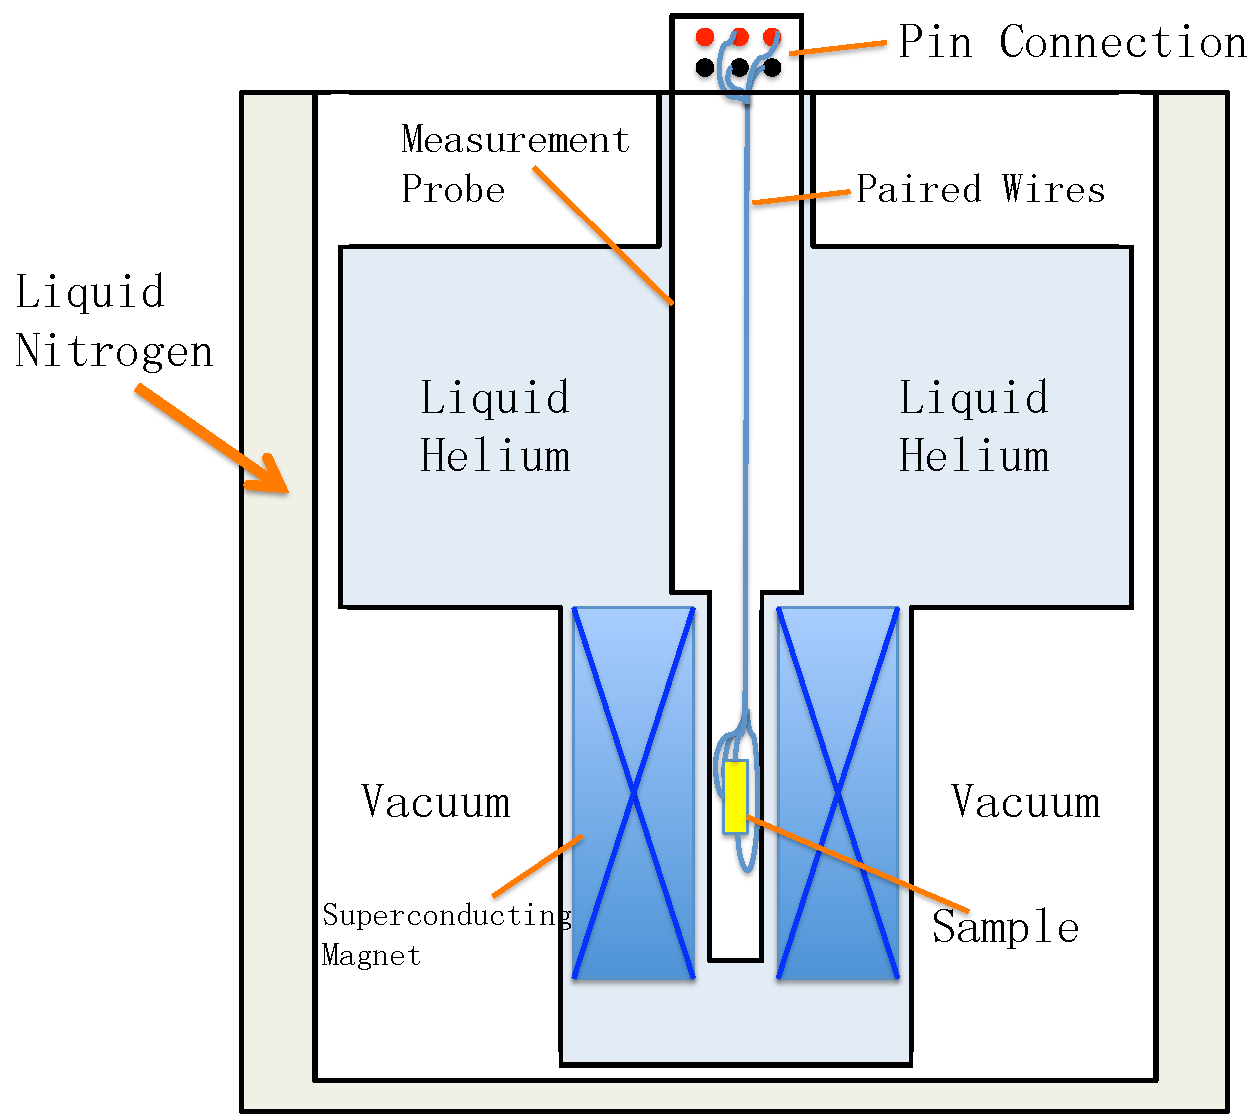
\includegraphics[width=0.8\linewidth]{ch-expsetup/figures/Magnet14T.pdf}
\caption{\label{Magnet14T}
A sketch of a typical in-house superconducting magnet with a measurement probe inside.}
  \end{center}
\end{figure}

Our in-house magnets are similar in their structures as shown in Fig. \ref{Magnet14T}. Each magnet has a dense coil made out of superconducting materials. The coil, with a bore for the measurement probe, is immersed by liquid helium in a dewar with a vacuum jacket. Outside the vacuum jacket, there is a liquid nitrogen jacket in order to reduce the thermal radiation from the helium container. The coil has a critical temperature higher than 4.2 K, and thus the coil will stay in the superconducting state when the current is flowing inside. The current is driven by an outside power supply. 

\subsection{Transport Measurement}\label{transport}

%talk about Sample Sample method
To make ohmic contacts to the samples, we typically use the silver paint from Dupont and thin gold wires to connect the sample to the measurement pads on the sample stage. To measure the magnetoresistance at tilted magnetic fields, we leverage our home-made rotation probe and the rotation probe that accompanies PPMS to rotate the sample in a magnetic field. Our home-made rotation probe has a Hall probe to tell the angle relative to the direction of the magnetic field. It can reach a temperature as low as 4.5 K, while PPMS's rotation probe can get to 2 K. To measure the transport property below 4 K, we use the He3 inserts from Oxford, Janis and IceOxford to to attain 0.3 K. Besides, NHMFL provides measurement inserts for both 4K-above and 4K-below transport measurements in the high-field experiments. To stabilize the temperature, we use the Lakeshore 340 temperature controller to adjust the heating power on the sample stage. 

The resistivity transport measurements were accomplished in different ways, such as by the lock-in technique and the delta-mode method. In the PPMS, we use the DC Resistivity mode (which is actually a delta mode) to measure the magnetoresistance. To measure the sample resistance in our in-house superconducting magnet, we typically use the SR830 Lock-in Amplifier from Stanford Research to implement the lock-in measurement, or use Keithley's 6221 current source and 2182A nano voltmeter for the delta-mode method. The choice depends on the sample's resistance as well as its contact resistance. Besides, the current through the sample is carefully chosen so that it has a large signal-to-noise ratio and does not increase the sample temperature. 

The Hall measurement is conducted in a way similar to the resistance measurement. But one noticeable detail is the method to measure the temperature dependence of the Hall coefficient. Here we implement the reciprocal technique set up by Sample et.al.\cite{Sample1987}. This method leverages the reciprocal theorem in electrodynamics so that the magnetic field does not need to be flipped during the Hall measurement. 

The main idea in Sample's work\cite{Sample1987} is as the following. Suppose there is a sample with four contact leads labeled as 1, 2, 3 and 4 respectively. In a magnetic field pointing to the positive direction, we first measure the resistance $R_{12, 34} (+B)$ by sending a current through leads 1 and 2, while measuring the voltage on leads 3 and 4. When we reverse the field direction, $R_{34, 12} (-B)$ denotes the resistance measured across the leads 1 and 2 with the current flowing through the leads 3 and 4. And the reciprocal theorem gives $R_{12, 34} (+B) = R_{34, 12} (-B)$. Therefore, we can also obtain $R_{12, 34} (-B) = R_{34, 12} (+B)$. In a Hall measurement, we normally need both $R_{12, 34} (+B)$ and $R_{12, 34} (-B)$ to calculate the Hall signal by $R_{yx} (B) = (R_{12, 34} (+B) - R_{12, 34} (-B))/2$ so that the extra contribution from the longitudinal resistance can be neutralized. But this conventional way also requires a change of the field direction, which usually takes a long time. Here we replace $R_{12, 34} (-B)$ with $R_{34, 12} (+B)$, and obtain $R_{yx} (B) = (R_{12, 34} (+B) - R_{34, 12} (+B))/2$. As a result, we do not need to flip the magnetic field. Instead, we need to switch the current and voltage leads, which can be done quickly with an electric relay switch. Using this method, we are able to switch the the current and voltage leads at each temperature and then measure the Hall coefficient v.s. temperature curve in a short time. 

\section{Ionic Liquid Gating Technique}
\label{sec:expsetup:ionicliquid}

Ionic liquid gating technique is a novel gating approach. Similar to the traditional solid gating method, ionic liquid gating also leverages a thin capacitor to change the chemical potential on the surface of a sample. One plate of the capacitance is also the sample surface. But unlike the solid state gating, the other capacitance plate is one layer of ions in the ionic liquid. Besides, since the ions sit on top of the sample surface, the thickness of the capacitor is on the order of the atomic scale. Thus it provides a very large capacitance and leads to a powerful gating effect. Previously, Iwasa's group first demonstrated the power of ionic liquid on ZnO\cite{yuan2009ZnO}. Then together with Iwasa\cite{Yuan2011}, Ando \cite{Ando_liquid} and Tokura group\cite{Checkelsky_liquid}, we introduced this novel gating method into TI transport experiments\cite{Xiong2013}. We discuss some technical details of the ionic liquid gating experiments here. 

The ionic liquid we use is DEME-TFSI, comprised of cations (CH$_3$ CH$_2$ )$_2$ (CH$_2$ CH$_2$ OCH$_3$ )CH$_3$ N$^+$ and anions (CF$_3$SO$_2$)$_2$N$_-$. This ionic liquid has been proved to provide a powerful gating effect in previous experiments\cite{yuan2009ZnO, ye2010liquid}. Before using the liquid, we pump it at $25 \,^{\circ}{\rm C}$ for 2 hours in order to minimize any water content that can accelerate unfavorable chemical reactions. Then the sample, the ionic liquid and the gold gate plate are put into a sapphire container (as shown in Fig. \ref{ILcontain}), and are quickly loaded into the cryostat. Then the sample is fast cooled down to around 220 K to diminish any chemical reaction or damage that may happen to the sample before the liquid freezes. As displayed by Fig. \ref{ILcontain}, there is a gold plate at the bottom of the container that serves as the gate electrode. Above the ionic liquid melting temperature, when a gate voltage is applied between the sample and the gold plate, ions will move inside the liquid. If the gate voltage $V_G$ is positive, cations will drift away from the gate plate and come to the sample surface, while anions will leave the sample. As a result, there forms a thin layer of extra cations on the sample surface, and these ions will generate a strong electric field towards the sample and lift its chemical potential. 

Starting from 0 V, we then apply a gate voltage $V_G$ to the gold plate at a �gating temperature� around 220 K at a sweeping speed of approximately 1 V/min. After the planned $V_G$ is attained, the sample is quickly cooled to 160 K to reduce the possibility of chemical reactions. Then the sample and the liquid are cooled down to 4 K slowly (at 2 K/min) to reduce the stress on the sample and the contacts caused by the freezing ionic liquid. The cooling process has a possibility to damage the sample as we find that repeated freezing and thawing of the ionic liquid can snap the leads or the crystal itself. At 4 K, the large $E$-field induced by the frozen surface anion density $N_{ion}$ (1-4$\times 10^{14}$ cm$^{-2}$) creates a depletion layer that changes the chemical potential in the sample significantly.

Unfortunately, the large gating power is not free. It is more difficult to change the gating voltage with the ionic liquid than using the solid-state gating. Every time we change $V_G$, we need to slowly (at 2 K/min) warm up the sample to the "gating temperature" around 220 K and change $V_G$ by small steps. At the "gating temperature", a typical way to change $V_G$ is to change it in steps of $\sim$0.02 V every 5 to 10 seconds, while monitoring the transient current $I_{trans}$ (1-40 nA). The time spent at the "gating temperature" is typically 300-500 s. Then the sample is cooled down to 5 K with the gating voltage fixed as we discussed above. To minimize the sample damage, we start at $V_G$ = 0 V during the first cool-down, followed by measurements at increasingly negative $V_G$ until the sample fails (usually by a discharge event).  We emphasize that the changes to the resistivity $\rho$ and the Hall density $n_H$ are reversible (see below) as long as $|V_G|$ does not exceed a limit. Upon returning $V_G$ to 0 V, we could recover the same starting value of R (at 5 K) provided $|V_G|$  is kept below 2 V.

\begin{figure}[!htbp]
  \begin{center}
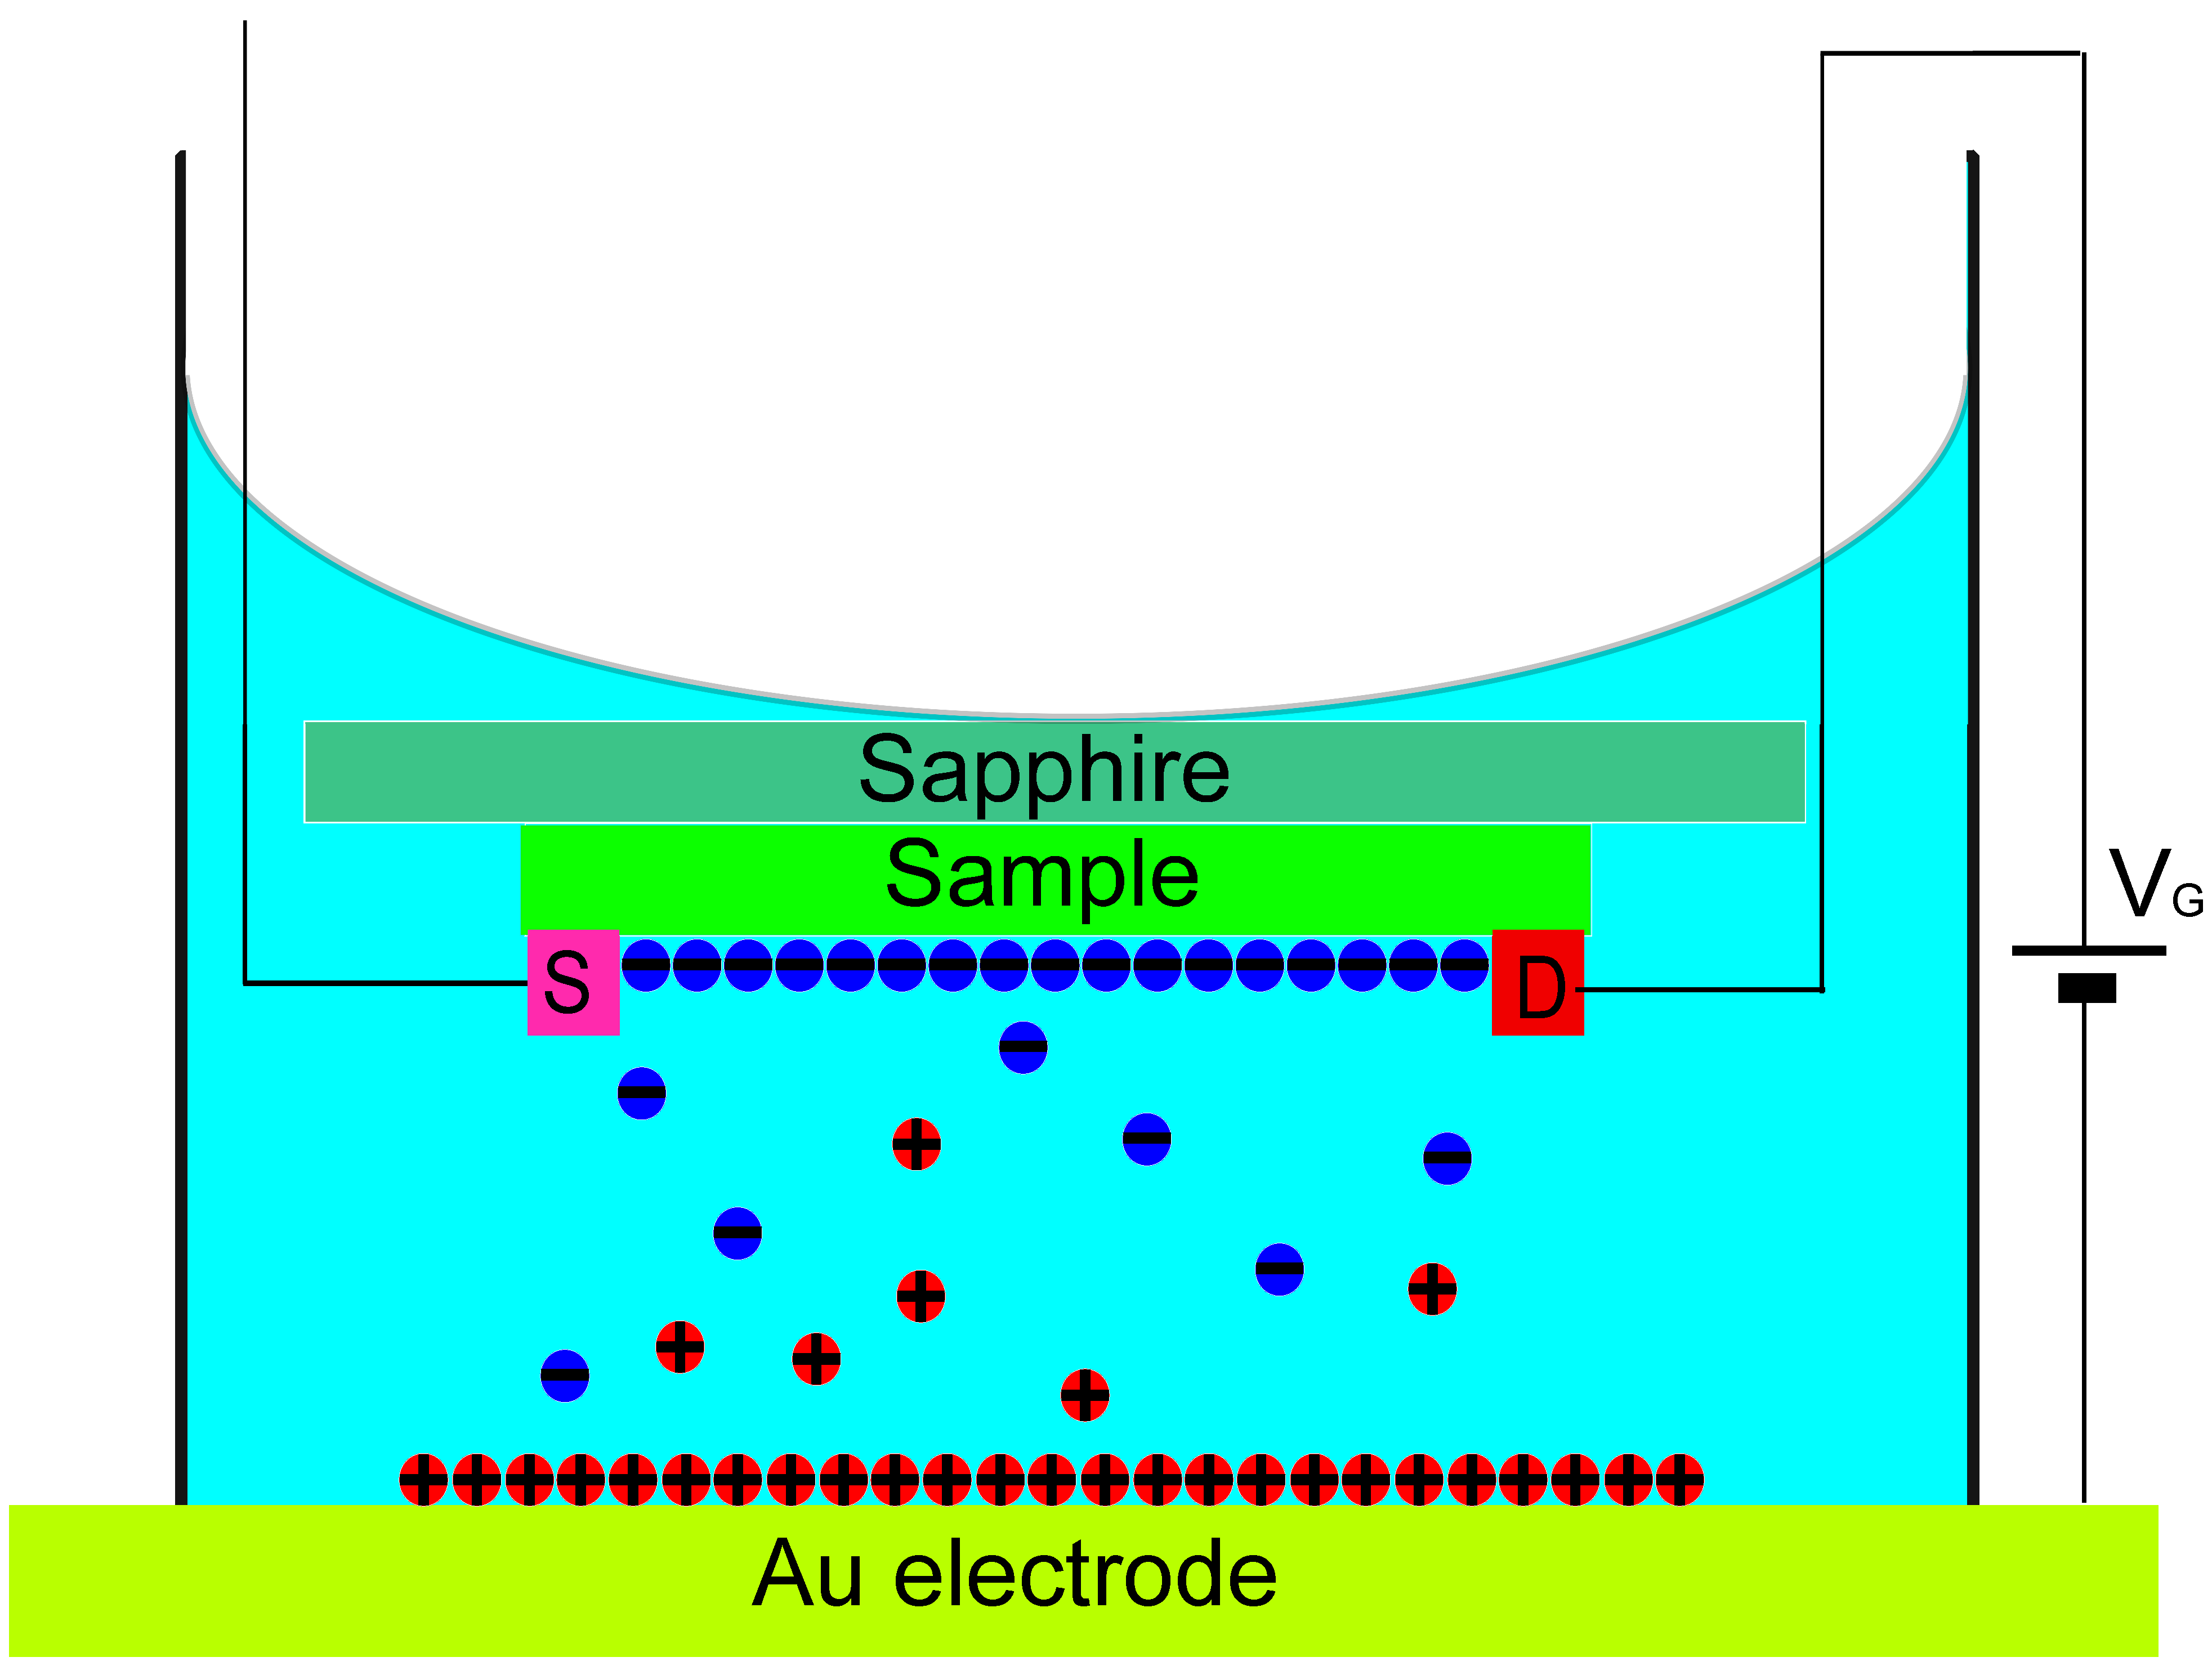
\includegraphics[width=0.8\linewidth]{ch-expsetup/figures/ILcontain.eps}
\caption{\label{ILcontain}
The configuration of the ionic liquid gating experiment. Both the ionic liquid and the sample are held in a sapphire container with a gold plate at the bottom. The Au plate is used to apply a gating voltage to the sample.}
  \end{center}
\end{figure}
\section{Protection of Air-sensitive Samples for Electric Measurement}
\label{sec:expsetup:airsensitive}

The Dirac semimetal Na$_3$Bi is an air-sensitive crystal. Due to the chemical reactivity of sodium, the whole Na$_3$Bi crystal can be easily oxidized in the air within ten seconds. Therefore, we need to make contacts to the sample within the glove box and then seal it well. The sample can only be loaded into the cryostat when it's isolated from any air or water. Great care should be taken during the process. Any remnant oxygen or water in the glove box, or any leaks in the seal can easily turn the crystal into ashes. 

Such fragileness of Na$_3$Bi crystals has created a large obstacle for us to make the electric contacts. To avoid any oxidization, we have to make contacts to the sample in the Argon glove box. Here we use silver epoxy (Epotek H20E) to fix the platinum wires on the crystals. We first put Pt wires and the silver epoxy on the right spot of the samle, then heat it at around 120 $\celsius$ for about 5 minutes so that the silver epoxy matures. Then we put the sample inside a small cylinder container as shown in Fig. \ref{Na3Bi_container} and connect the Pt wires to the electric pads on the cap of the container. We diminish the chance of oxidization by adding paratone oil inside the container after the sample is mounted. Thus the sample is completely immersed in the paratone oil. Then the container is sealed and put into a cryostat for the measurement. Our results show that the sample can survive inside the container for a couple of days even when the container is exposed to air. Once the crystal is loaded into a cryostat and stays below 100 K, the sample stays the same during a long time of measurement. Hence we are able to measure the same Na$_3$Bi sample in different cryostats for a long time.


\begin{figure}[!htbp]
  \begin{center}
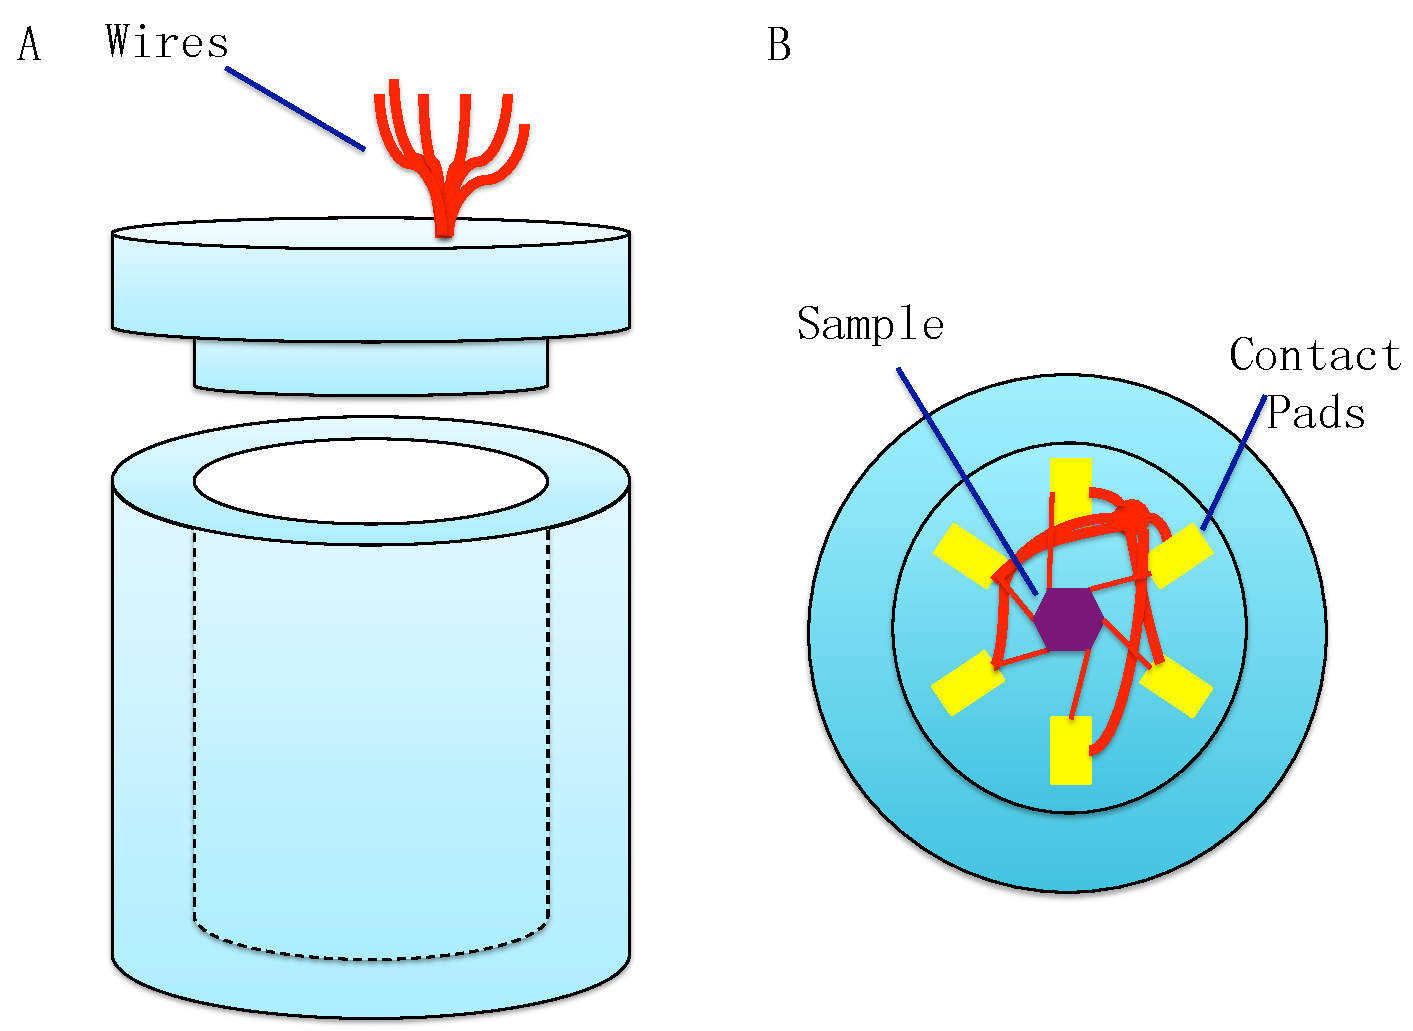
\includegraphics[width=0.8\linewidth]{ch-expsetup/figures/Na3Bi_container.pdf}
\caption{\label{Na3Bi_container}
A sketch of the container that we use to protect the Na$_3$Bi crystal. Panel (A) shows that the container has a bucket and a cap. There are wires  going through the cap. Before the seal, the main bucket is filled with paratone oil to prevent oxidization. Panel (B) shows that the sample is mounted on the inner side of the cap. There are Pt wires connecting the sample and the contact pads on the cap. 
}
  \end{center}
\end{figure}






